% Options for packages loaded elsewhere
\PassOptionsToPackage{unicode}{hyperref}
\PassOptionsToPackage{hyphens}{url}
\PassOptionsToPackage{dvipsnames,svgnames,x11names}{xcolor}
%
\documentclass[
  12pt,
  letterpaper,
  DIV=11,
  numbers=noendperiod]{scrartcl}

\usepackage{amsmath,amssymb}
\usepackage{lmodern}
\usepackage{iftex}
\ifPDFTeX
  \usepackage[T1]{fontenc}
  \usepackage[utf8]{inputenc}
  \usepackage{textcomp} % provide euro and other symbols
\else % if luatex or xetex
  \usepackage{unicode-math}
  \defaultfontfeatures{Scale=MatchLowercase}
  \defaultfontfeatures[\rmfamily]{Ligatures=TeX,Scale=1}
\fi
% Use upquote if available, for straight quotes in verbatim environments
\IfFileExists{upquote.sty}{\usepackage{upquote}}{}
\IfFileExists{microtype.sty}{% use microtype if available
  \usepackage[]{microtype}
  \UseMicrotypeSet[protrusion]{basicmath} % disable protrusion for tt fonts
}{}
\makeatletter
\@ifundefined{KOMAClassName}{% if non-KOMA class
  \IfFileExists{parskip.sty}{%
    \usepackage{parskip}
  }{% else
    \setlength{\parindent}{0pt}
    \setlength{\parskip}{6pt plus 2pt minus 1pt}}
}{% if KOMA class
  \KOMAoptions{parskip=half}}
\makeatother
\usepackage{xcolor}
\usepackage[margin=1in]{geometry}
\setlength{\emergencystretch}{3em} % prevent overfull lines
\setcounter{secnumdepth}{-\maxdimen} % remove section numbering
% Make \paragraph and \subparagraph free-standing
\ifx\paragraph\undefined\else
  \let\oldparagraph\paragraph
  \renewcommand{\paragraph}[1]{\oldparagraph{#1}\mbox{}}
\fi
\ifx\subparagraph\undefined\else
  \let\oldsubparagraph\subparagraph
  \renewcommand{\subparagraph}[1]{\oldsubparagraph{#1}\mbox{}}
\fi

\usepackage{color}
\usepackage{fancyvrb}
\newcommand{\VerbBar}{|}
\newcommand{\VERB}{\Verb[commandchars=\\\{\}]}
\DefineVerbatimEnvironment{Highlighting}{Verbatim}{commandchars=\\\{\}}
% Add ',fontsize=\small' for more characters per line
\usepackage{framed}
\definecolor{shadecolor}{RGB}{241,243,245}
\newenvironment{Shaded}{\begin{snugshade}}{\end{snugshade}}
\newcommand{\AlertTok}[1]{\textcolor[rgb]{0.68,0.00,0.00}{#1}}
\newcommand{\AnnotationTok}[1]{\textcolor[rgb]{0.37,0.37,0.37}{#1}}
\newcommand{\AttributeTok}[1]{\textcolor[rgb]{0.40,0.45,0.13}{#1}}
\newcommand{\BaseNTok}[1]{\textcolor[rgb]{0.68,0.00,0.00}{#1}}
\newcommand{\BuiltInTok}[1]{\textcolor[rgb]{0.00,0.23,0.31}{#1}}
\newcommand{\CharTok}[1]{\textcolor[rgb]{0.13,0.47,0.30}{#1}}
\newcommand{\CommentTok}[1]{\textcolor[rgb]{0.37,0.37,0.37}{#1}}
\newcommand{\CommentVarTok}[1]{\textcolor[rgb]{0.37,0.37,0.37}{\textit{#1}}}
\newcommand{\ConstantTok}[1]{\textcolor[rgb]{0.56,0.35,0.01}{#1}}
\newcommand{\ControlFlowTok}[1]{\textcolor[rgb]{0.00,0.23,0.31}{#1}}
\newcommand{\DataTypeTok}[1]{\textcolor[rgb]{0.68,0.00,0.00}{#1}}
\newcommand{\DecValTok}[1]{\textcolor[rgb]{0.68,0.00,0.00}{#1}}
\newcommand{\DocumentationTok}[1]{\textcolor[rgb]{0.37,0.37,0.37}{\textit{#1}}}
\newcommand{\ErrorTok}[1]{\textcolor[rgb]{0.68,0.00,0.00}{#1}}
\newcommand{\ExtensionTok}[1]{\textcolor[rgb]{0.00,0.23,0.31}{#1}}
\newcommand{\FloatTok}[1]{\textcolor[rgb]{0.68,0.00,0.00}{#1}}
\newcommand{\FunctionTok}[1]{\textcolor[rgb]{0.28,0.35,0.67}{#1}}
\newcommand{\ImportTok}[1]{\textcolor[rgb]{0.00,0.46,0.62}{#1}}
\newcommand{\InformationTok}[1]{\textcolor[rgb]{0.37,0.37,0.37}{#1}}
\newcommand{\KeywordTok}[1]{\textcolor[rgb]{0.00,0.23,0.31}{#1}}
\newcommand{\NormalTok}[1]{\textcolor[rgb]{0.00,0.23,0.31}{#1}}
\newcommand{\OperatorTok}[1]{\textcolor[rgb]{0.37,0.37,0.37}{#1}}
\newcommand{\OtherTok}[1]{\textcolor[rgb]{0.00,0.23,0.31}{#1}}
\newcommand{\PreprocessorTok}[1]{\textcolor[rgb]{0.68,0.00,0.00}{#1}}
\newcommand{\RegionMarkerTok}[1]{\textcolor[rgb]{0.00,0.23,0.31}{#1}}
\newcommand{\SpecialCharTok}[1]{\textcolor[rgb]{0.37,0.37,0.37}{#1}}
\newcommand{\SpecialStringTok}[1]{\textcolor[rgb]{0.13,0.47,0.30}{#1}}
\newcommand{\StringTok}[1]{\textcolor[rgb]{0.13,0.47,0.30}{#1}}
\newcommand{\VariableTok}[1]{\textcolor[rgb]{0.07,0.07,0.07}{#1}}
\newcommand{\VerbatimStringTok}[1]{\textcolor[rgb]{0.13,0.47,0.30}{#1}}
\newcommand{\WarningTok}[1]{\textcolor[rgb]{0.37,0.37,0.37}{\textit{#1}}}

\providecommand{\tightlist}{%
  \setlength{\itemsep}{0pt}\setlength{\parskip}{0pt}}\usepackage{longtable,booktabs,array}
\usepackage{calc} % for calculating minipage widths
% Correct order of tables after \paragraph or \subparagraph
\usepackage{etoolbox}
\makeatletter
\patchcmd\longtable{\par}{\if@noskipsec\mbox{}\fi\par}{}{}
\makeatother
% Allow footnotes in longtable head/foot
\IfFileExists{footnotehyper.sty}{\usepackage{footnotehyper}}{\usepackage{footnote}}
\makesavenoteenv{longtable}
\usepackage{graphicx}
\makeatletter
\def\maxwidth{\ifdim\Gin@nat@width>\linewidth\linewidth\else\Gin@nat@width\fi}
\def\maxheight{\ifdim\Gin@nat@height>\textheight\textheight\else\Gin@nat@height\fi}
\makeatother
% Scale images if necessary, so that they will not overflow the page
% margins by default, and it is still possible to overwrite the defaults
% using explicit options in \includegraphics[width, height, ...]{}
\setkeys{Gin}{width=\maxwidth,height=\maxheight,keepaspectratio}
% Set default figure placement to htbp
\makeatletter
\def\fps@figure{htbp}
\makeatother
\newlength{\cslhangindent}
\setlength{\cslhangindent}{1.5em}
\newlength{\csllabelwidth}
\setlength{\csllabelwidth}{3em}
\newlength{\cslentryspacingunit} % times entry-spacing
\setlength{\cslentryspacingunit}{\parskip}
\newenvironment{CSLReferences}[2] % #1 hanging-ident, #2 entry spacing
 {% don't indent paragraphs
  \setlength{\parindent}{0pt}
  % turn on hanging indent if param 1 is 1
  \ifodd #1
  \let\oldpar\par
  \def\par{\hangindent=\cslhangindent\oldpar}
  \fi
  % set entry spacing
  \setlength{\parskip}{#2\cslentryspacingunit}
 }%
 {}
\usepackage{calc}
\newcommand{\CSLBlock}[1]{#1\hfill\break}
\newcommand{\CSLLeftMargin}[1]{\parbox[t]{\csllabelwidth}{#1}}
\newcommand{\CSLRightInline}[1]{\parbox[t]{\linewidth - \csllabelwidth}{#1}\break}
\newcommand{\CSLIndent}[1]{\hspace{\cslhangindent}#1}

\usepackage{booktabs}
\usepackage{longtable}
\usepackage{array}
\usepackage{multirow}
\usepackage{wrapfig}
\usepackage{float}
\usepackage{colortbl}
\usepackage{pdflscape}
\usepackage{tabu}
\usepackage{threeparttable}
\usepackage{threeparttablex}
\usepackage[normalem]{ulem}
\usepackage{makecell}
\usepackage{xcolor}
\KOMAoption{captions}{tableheading}
\makeatletter
\makeatother
\makeatletter
\makeatother
\makeatletter
\@ifpackageloaded{caption}{}{\usepackage{caption}}
\AtBeginDocument{%
\ifdefined\contentsname
  \renewcommand*\contentsname{Table of contents}
\else
  \newcommand\contentsname{Table of contents}
\fi
\ifdefined\listfigurename
  \renewcommand*\listfigurename{List of Figures}
\else
  \newcommand\listfigurename{List of Figures}
\fi
\ifdefined\listtablename
  \renewcommand*\listtablename{List of Tables}
\else
  \newcommand\listtablename{List of Tables}
\fi
\ifdefined\figurename
  \renewcommand*\figurename{Figure}
\else
  \newcommand\figurename{Figure}
\fi
\ifdefined\tablename
  \renewcommand*\tablename{Table}
\else
  \newcommand\tablename{Table}
\fi
}
\@ifpackageloaded{float}{}{\usepackage{float}}
\floatstyle{ruled}
\@ifundefined{c@chapter}{\newfloat{codelisting}{h}{lop}}{\newfloat{codelisting}{h}{lop}[chapter]}
\floatname{codelisting}{Listing}
\newcommand*\listoflistings{\listof{codelisting}{List of Listings}}
\makeatother
\makeatletter
\@ifpackageloaded{caption}{}{\usepackage{caption}}
\@ifpackageloaded{subcaption}{}{\usepackage{subcaption}}
\makeatother
\makeatletter
\@ifpackageloaded{tcolorbox}{}{\usepackage[many]{tcolorbox}}
\makeatother
\makeatletter
\@ifundefined{shadecolor}{\definecolor{shadecolor}{rgb}{.97, .97, .97}}
\makeatother
\makeatletter
\makeatother
\ifLuaTeX
  \usepackage{selnolig}  % disable illegal ligatures
\fi
\IfFileExists{bookmark.sty}{\usepackage{bookmark}}{\usepackage{hyperref}}
\IfFileExists{xurl.sty}{\usepackage{xurl}}{} % add URL line breaks if available
\urlstyle{same} % disable monospaced font for URLs
\hypersetup{
  pdftitle={Katabuchi et al., Decomposing leaf mass into metabolic and structural components explains divergent patterns of trait variation within and among plant species},
  colorlinks=true,
  linkcolor={blue},
  filecolor={Maroon},
  citecolor={Blue},
  urlcolor={Blue},
  pdfcreator={LaTeX via pandoc}}

\title{Katabuchi et al., Decomposing leaf mass into metabolic and
structural components explains divergent patterns of trait variation
within and among plant species}
\author{}
\date{}

\begin{document}
\maketitle
\ifdefined\Shaded\renewenvironment{Shaded}{\begin{tcolorbox}[boxrule=0pt, interior hidden, breakable, borderline west={3pt}{0pt}{shadecolor}, enhanced, frame hidden, sharp corners]}{\end{tcolorbox}}\fi

\renewcommand*\contentsname{Table of contents}
{
\hypersetup{linkcolor=}
\setcounter{tocdepth}{3}
\tableofcontents
}
\newpage

\hypertarget{appendix-s1-prior-information}{%
\section{Appendix S1: Prior
information}\label{appendix-s1-prior-information}}

The logarithms of \emph{A}\textsubscript{area},
\emph{R}\textsubscript{area}, and LL for leaf sample \emph{i} were
assumed to have a multivariate normal distribution as following:

\begin{align}
\left(
\begin{array}{ccc}
\mathrm{ln}(A_{\mathrm{area} \, i})\\
\mathrm{ln}(R_{\mathrm{area} \, i}) \\
\mathrm{ln}(\mathrm{LL}_i)
\end{array}
\right)
\sim \mathrm{MVN}
\left(
\begin{array}{rrr}
\mathrm{E}[A_{\mathrm{area} \, i}]\\
\mathrm{E}[R_{\mathrm{area} \, i}] &, \boldsymbol{\Sigma}\\
\mathrm{E}[\mathrm{LL}_i]
\end{array}
\right) \tag{S1}
\end{align}

where E{[}\(\cdot\){]} indicates expected value; \(\boldsymbol{\Sigma}\)
indicates a covariance matrix. Expected values are based on Eqs. 1-6 in
the main text.

We used non-informative or weakly informative prior distributions
(\protect\hyperlink{ref-Lemoine2019}{Lemoine 2019}). The covariance
mkatrix in Eq. S1 was decomposed as
\({\mathbf \Sigma} = {\mathrm diag}({\mathbf \sigma}){\mathbf \Omega}{\mathrm diag}({\mathbf \sigma}) = {\mathrm diag}({\mathbf \sigma}){\mathbf L}{\mathbf L}\prime {\mathrm diag}({\mathbf \sigma})\)
using a Cholesky decomposition, where \({\mathbf \sigma}\) is a vector
of \(\sigma_{1}\), \(\sigma_{2}\), and \(\sigma_{3}\);
\({\mathbf \Omega}\) is a correlation matrix of \(\rho_{12}\),
\(\rho_{13}\), and \(\rho_{23}\); and \textbf{L} is a lower triangular
matrix. Instead of assigning prior distributions on directly, priors
were assigned on and \textbf{L} to avoid a strong dependence between and
(\protect\hyperlink{ref-Lewandowski2009}{Lewandowski et al. 2009},
\protect\hyperlink{ref-Alvarez2014}{Alvarez et al. 2014}). A prior for
\textbf{L} was specified as a so-called LKJ distribution with shape
parameter 2 (\protect\hyperlink{ref-Lewandowski2009}{Lewandowski et al.
2009}), which is weakly informative for the correlation matrix. A prior
for \({\mathrm diag}({\mathbf \sigma})\) was specified as a Half-Cauchy
distribution with location 0 and scale 5, which is weakly informative
and allows for occasional large coefficients while still performing a
reasonable amount of shrinkage for coefficients near zero
(\protect\hyperlink{ref-Gelman2008}{Gelman et al. 2008}). A prior for
\(\mathbf{\sigma}\) was specified as a Half-Cauchy distribution with
location 0 and scale 5, which is weakly informative and allows for
occasional large coefficients while still performing a reasonable amount
of shrinkage for coefficients near zero
(\protect\hyperlink{ref-Gelman2008}{Gelman et al. 2008}). Priors for
\(\alpha_{0,p,s}\), \(\beta_{0,p,s}\), and \(\gamma_{0,p,s}\) in Eqs.
4-6 were weakly informative and specified as normal distributions with
mean 0 and standard deviation 5. Priors for \emph{f\textsubscript{i}} in
Eqs. 4-6 were non-informative and specified as uniform distributions
with range (0, 1).

\newpage

\hypertarget{appendix-s2-randomization-including-table-as1-and-figure-as1}{%
\section{Appendix S2: Randomization (including Table AS1 and Figure
AS1)}\label{appendix-s2-randomization-including-table-as1-and-figure-as1}}

We generated 10 randomized datasets for each of the GLOPNET and the
Panama datasets by shuffling each trait value across leaf samples, and
fit the best models (Appendix S1) to the randomized data.

\hypertarget{table-as1}{%
\subsection{Table AS1}\label{table-as1}}

\begin{itemize}
\tightlist
\item
  No\_large\_Rhat: The number of parameters (including transformed
  parameters) that shows Rhat (Gelman-Rubin statistic) greater than
  1.05.
\item
  No\_divergence: The number of iterations that shows divergent
  transitions.
\end{itemize}

\begin{longtable}[]{@{}lrrr@{}}
\toprule()
Data & Simulation\_ID & No\_large\_Rhat & No\_divergence \\
\midrule()
\endhead
GLOPNET & 1 & 239 & 2 \\
GLOPNET & 2 & 78 & 4 \\
GLOPNET & 3 & 14 & 0 \\
GLOPNET & 4 & 420 & 0 \\
GLOPNET & 5 & 13 & 1 \\
GLOPNET & 6 & 4 & 0 \\
GLOPNET & 7 & 1 & 0 \\
GLOPNET & 8 & 10 & 0 \\
GLOPNET & 9 & 19 & 1 \\
GLOPNET & 10 & 228 & 22 \\
Panama & 1 & 784 & 103 \\
Panama & 2 & 606 & 40 \\
Panama & 3 & 687 & 19 \\
Panama & 4 & 616 & 101 \\
Panama & 5 & 726 & 0 \\
Panama & 6 & 752 & 225 \\
Panama & 7 & 771 & 69 \\
Panama & 8 & 680 & 18 \\
Panama & 9 & 832 & 28 \\
Panama & 10 & 681 & 18 \\
\bottomrule()
\end{longtable}

Model results obtained from the randomized datasets did not convergent
based on the Gelman-Rubin statistic or showed divergent transitions.

\newpage

\hypertarget{figure-as1}{%
\subsection{Figure AS1}\label{figure-as1}}

Although many parameters showed large Rhat values, which suggests that
the posterior distributions were not converged well, we checked the
regression coefficients for GLOPNET (\(\alpha_{0, p, s}\),
\(\beta_{0, s}\), and \(\gamma_{0, p, s}\) in Eqs. 4-6 in the main
text). There are 10 independent simulations (randomizations) in total.
The scaling parameters in the randomized datasets did not show any
patterns. Thus, the tests with randomized data indicate that our model
is not inherently prone to overfitting or to producing patterns from
noise. \includegraphics{../figs/coef_rand.png}

\newpage

\hypertarget{appendix-s3-simulation-for-mass-dependency-of-aarea}{%
\section{\texorpdfstring{Appendix S3: Simulation for mass dependency of
\emph{A}\textsubscript{area}}{Appendix S3: Simulation for mass dependency of Aarea}}\label{appendix-s3-simulation-for-mass-dependency-of-aarea}}

To simulate mass dependency of \emph{A}\textsubscript{area}, we
generated LMAp and LMAs values for leaf sample \emph{i} using normal
distibutions (N) for GLPONET and sun leaves of Panama with a sample size
of 100:

\[
\mathrm{ln}(\mathrm{LMAp}_{i}) \sim N(\mathrm{ln}(\mu_p), \sigma_p)
\]

\[
\mathrm{ln}(\mathrm{LMAs}_{i}) \sim N(\mathrm{ln}(\mu_s), \sigma_s)
\]

where \(\mu_p\) and \(\mu_s\) are the mean of LMAp and LMAs on the
log-scale, respectively, and \(\sigma_p\) and \(\sigma_s\) are the
standard deviation of LMAp and LMAs on the log-scale, respectively.

Because there was a weak negative correlation between LMAp and LMAs
values of shade leaves in Panama, LMAp and LMAs values were generated
using a multivairate normal distribution (MVN):

\[
\begin{bmatrix}
\mathrm{ln}(\mathrm{LMAp}_{i})\\
\mathrm{ln}(\mathrm{LMAs}_{i})
\end{bmatrix}
\sim \mathrm{MVN}
\left[
\begin{matrix}
\ln(\mu_{p})\\
\ln(\mu_{s})
\end{matrix}
,\mathbf{\Sigma}
\right]
\]

\[
\mathbf{\Sigma} = \
\begin{bmatrix}
\sigma_p^2 & \rho \sigma_p \sigma_s \\
\rho \sigma_p \sigma_s & \sigma_s^2 \\
\end{bmatrix}
\]

where \(\Sigma\) is the covariance matrix of ln(LMAp) and ln(LMAs),
\(\rho\) is the correlation coefficient between ln(LMAp) and ln(LMAs).

We used the empirical estimates for \(\mu_p\), \(\mu_s\), \(\sigma_p\),
and \(\rho\) while with changing \(\sigma_s\) between ln(1.01) and
ln(10). \emph{A}\textsubscript{area} was then generated based the values
obtianed from the above simulation:

\[
\mathrm{ln}(A_{\mathrm{area} \, i}) = \mathrm{ln}(\alpha_0) + \alpha_p\mathrm{ln}(\mathrm{LMAp}_{i}) + \alpha_s\mathrm{ln}(\mathrm{LMAs}_{i}).
\]

Parameter settings are as following, GLOPNET: \(\mu_p\) = 58.8,
\(\mu_s\) = 63.1, \(\sigma_p\) = 2.12, \(\alpha_p\) = 0.28, \(\alpha_s\)
= -0.13, sun leaves in Panama: \(\mu_p\) = 45.7, \(\mu_s\) = 30.6,
\(\sigma_p\) = 1.51, and \(\alpha_p\) = 0.56, \(\alpha_s\) = 0, shade
leaves in Panama: \(\mu_p\) = 8.4, \(\mu_s\) = 24.5, \(\sigma_p\) =
1.84, \(\alpha_p\) = 0.56, \(\alpha_s\) = 0, \(\rho\) = -0.4.

We finally calculated mass dependicy (\emph{b}) using the following
ordinary least square regression:

\[
\mathrm{ln}(A_{\mathrm{area} \, i}) = \mathrm{ln}(a) + b \mathrm{ln}(\mathrm{LMA}_{i}).
\]

We repeated these steps 1000 times.

\newpage

\hypertarget{figure-s1}{%
\section{Figure S1}\label{figure-s1}}

\begin{figure}

{\centering 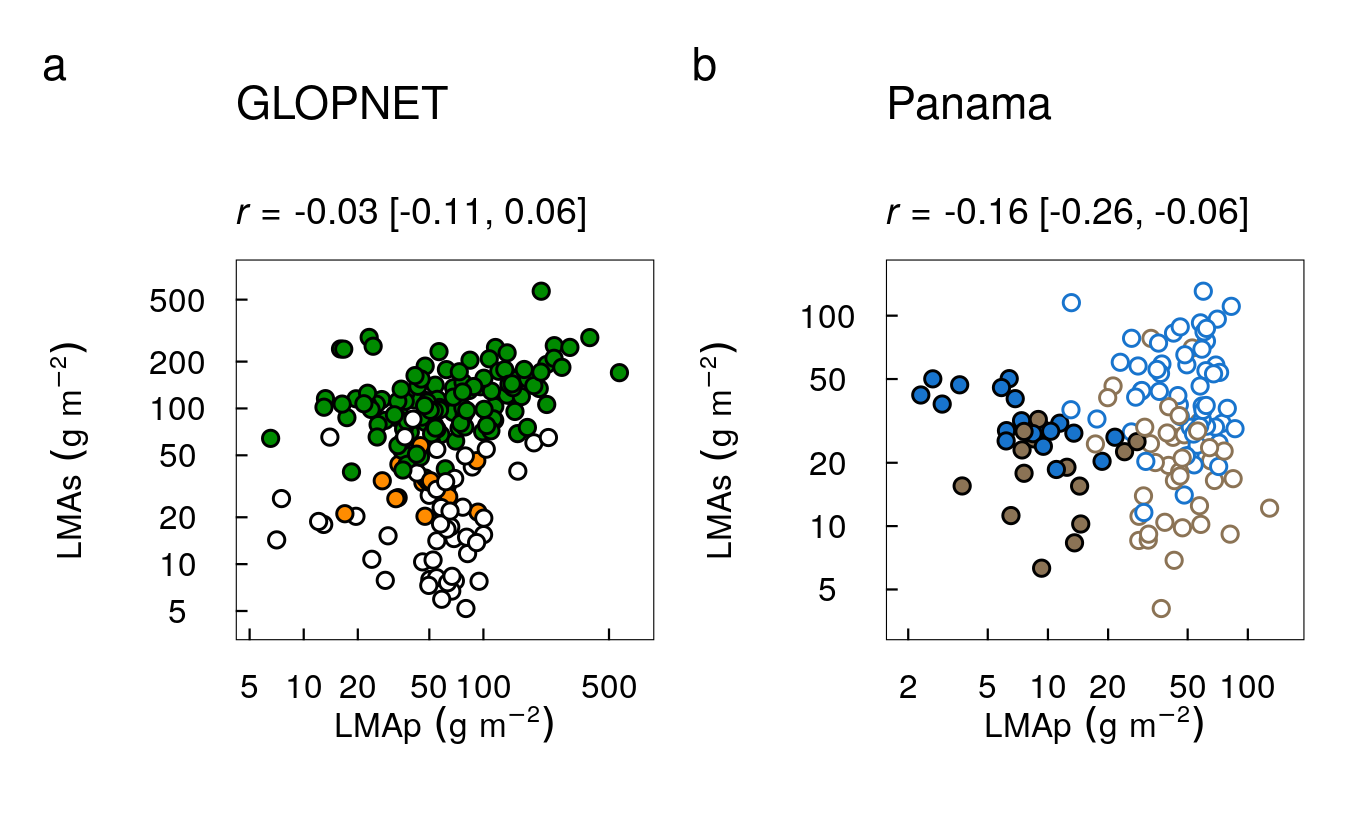
\includegraphics{../figs/ps_point.png}

}

\caption{\label{fig-LMAp_LMAs}Pearson correlation coefficients for
posterior medians of LMAp vs LMAs in the (a) GLOPNET and (b) Panama
datasets. The non-significant or weak \emph{r} values indicate that a
single axis could not accurately represent the two-dimensional space.
Symbols as in Main Text Figs. 1-2.}

\end{figure}

\newpage

\hypertarget{figure-s2}{%
\section{Figure S2}\label{figure-s2}}

\begin{figure}

{\centering \includegraphics{../figs/box_inter.png}

}

\caption{\label{fig-box_inter}Boxplots comparing leaf mass per area
(LMA), photosynthetic leaf mass per area (LMAp; posterior means), and
structural leaf mass per area (LMAs; posterior means) across sites (wet
and dry) and canopy strata (sun and shade) in Panama. The results shown
here include all leaves in the Panama dataset, whereas Fig. 5 in the
main text only includes Panama species for which both sun and shade
leaves were available. Boxplot symbols as in Fig. 5. Groups sharing the
same letters are not significantly different (P \textgreater{} 0.05;
t-tests).}

\end{figure}

\newpage

\hypertarget{figure-s3}{%
\section{Figure S3}\label{figure-s3}}

\begin{figure}

{\centering 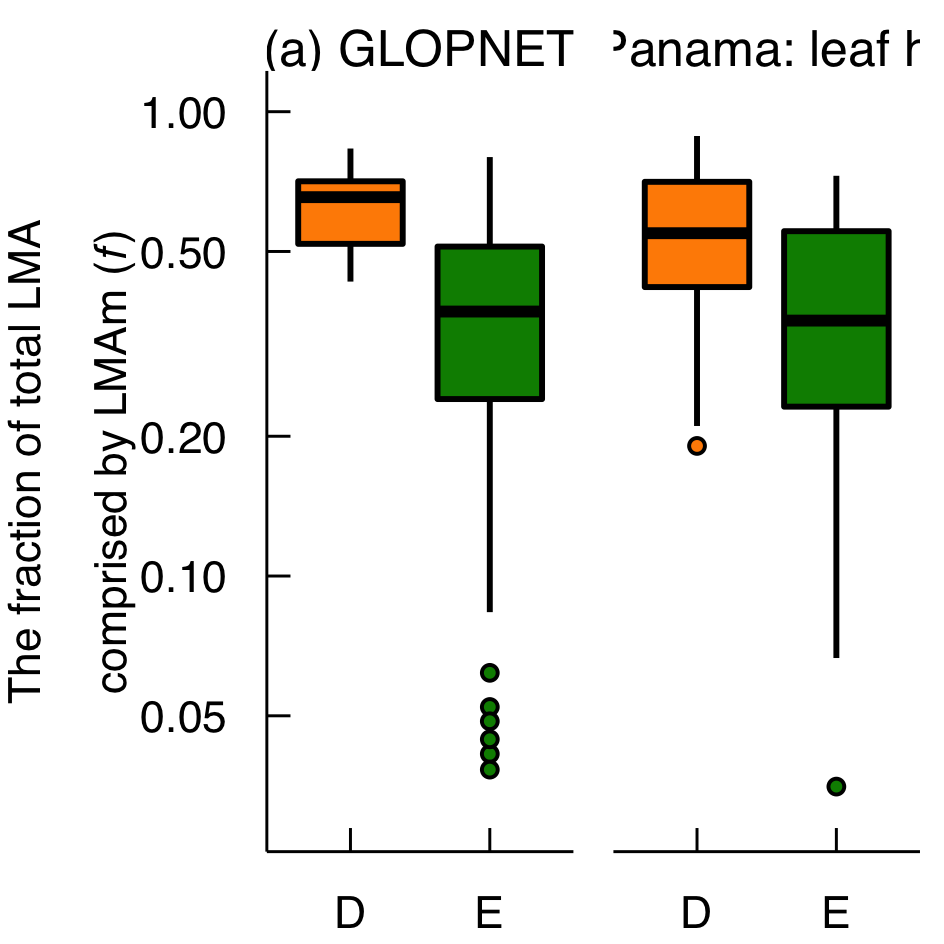
\includegraphics{../figs/box_frac.png}

}

\caption{\label{fig-box_frac}Boxplots comparing posterior medians of the
latent variable f (the fraction of total LMA comprised by LMAm) across
deciduous (D) and evergreen (E) leaves in GLOPNET and Panama, and across
sites (wet and dry) and canopy strata (sun and shade) in Panama. Note
that LMAm = f × LMA, and LMAs = (1 -- f) × LMA. (a) Deciduous and
evergreen leaves in the GLOPNET dataset; (b) deciduous and evergreen
leaves for Panama species for which both sun and shade leaves were
available; (c) leaves for Panama species for which both sun and shade
leaves were available; and (d) all leaves for Panama. At the dry Panama
site, the increase in LMA from shade to sun (Fig. 4) is due to roughly
equal proportional increases in LMAm and LMAs (because f is similar
between sun and shade), whereas at the wet Panama site, the increase in
LMA from shade to sun (Fig. 4) is due primarily to increased LMAm
(because f is greater in sun than shade). GLOPNET results are for the
Potential LL Model (Eq. 5), and Panama results are for the Optimal LL
Model with site effects (Eq. 13 and Supporting Information, Section
3.1). The center line in each box indicates the median, upper and lower
box edges indicate the interquartile range, whiskers show 1.5 times the
interquartile range, and points are outliers. Groups sharing the same
letters are not significantly different (P \textgreater{} 0.05;
t-tests).''\}}

\end{figure}

\newpage

\hypertarget{figure-s4}{%
\section{Figure S4}\label{figure-s4}}

\begin{figure}

{\centering \includegraphics{../figs/mass_prop_sim.png}

}

\caption{\label{fig-mass_prop_sim}The relationships between mass
dependency (\emph{b} in Eq. 5 in the main text) and relative variance in
LMAs to LMA for the different ranges of the scaling exponent
\(\alpha_p\) and \(\alpha_s\). \textbf{a}, the scaling exponent
\(\alpha_p\) vary from 0.1 to 1.0 while the scaling exponent
\(\alpha_s\) is constant (\(\alpha_s\) = -0.13,). \textbf{b}, the
scaling exponent \(\alpha_s\) vary from -0.5 to 0.5 while the scaling
exponent \(\alpha_p\) is constant (\(\alpha_p\) = 0.28,). Solid lines
indicate simulated means and shaded regions indicate 95\% CI. The
photosynthetic rate (\emph{A}\textsubscript{max}) is primarily
mass-dependent (\emph{b} \textgreater{} 0.5), primarily area-dependent
(0.5 \textgreater{} \emph{b} \textgreater{} 0) and purely area-dependent
(\emph{b} = 0) (\protect\hyperlink{ref-Osnas2018}{Osnas et al. 2018}).
Note that when \emph{b} \textgreater{} 1, \emph{A}\textsubscript{area}
dramatically increase with LMA, which is not realistic. Parameter
settings: \(\alpha_0\) = 1.77, \(\mu_p\) = 58.8, \(\mu_s\) = 63.1,
\(\sigma_p\) = 2.12.}

\end{figure}

\newpage

\hypertarget{figure-s5}{%
\section{Figure S5}\label{figure-s5}}

\begin{figure}

{\centering \includegraphics{../figs/mass_prop_comp.png}

}

\caption{\label{fig-mass_prop_comp}The relationships between mass
dependency (\emph{b} in Eq. 5 in the main tex) and relative variance in
LMAs to LMA for the simulated dataset gerenated by a normal distribution
(N) and a multivariate normal distribution (MVN). Parameter settings:
\(\alpha_0\) = 0.33, \(\alpha_p\) = 0.56, \(\alpha_s\) = 0, \(\mu_p\) =
8.4, \(\mu_s\) = 24.5, \(\sigma_p\) = 1.84, and \(\rho\) = -0.4,}

\end{figure}

\newpage

\hypertarget{figure-s6}{%
\section{Figure S6}\label{figure-s6}}

\begin{figure}

{\centering 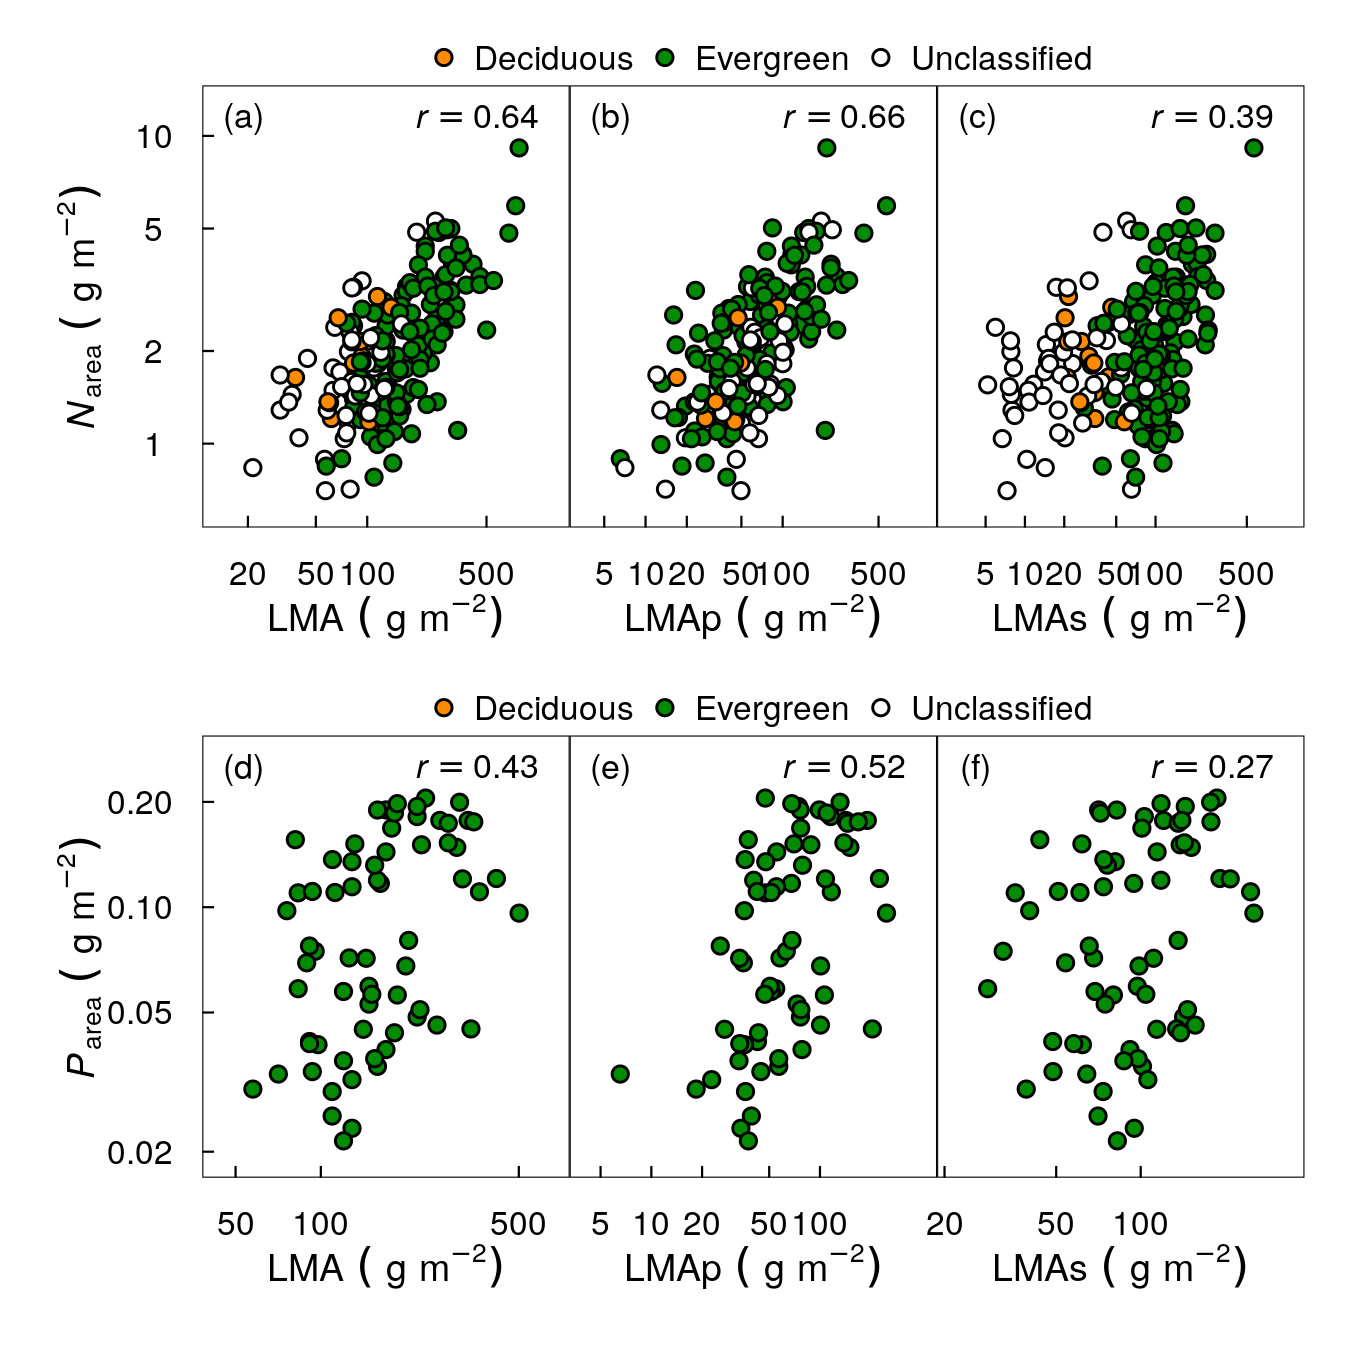
\includegraphics{../figs/gl_point_np2.png}

}

\caption{\label{fig-glnp}Measured traits related to photosynthesis and
metabolism (nitrogen and phosphorus per-unit leaf area;
\emph{N}\textsubscript{area} and \emph{P}\textsubscript{area}) are
positively correlated with LMA and with estimates (posterior means) of
the photosynthetic and structural LMA components (LMAp and LMAs,
respectively) in the GLOPNET dataset. LMAp yields more consistent
relationships compared to LMA and LMAs; e.g., evergreen and deciduous
leaves align along a single relationship in panel b, but not in panels a
or c.}

\end{figure}

\hypertarget{appendix-s4-stan-code}{%
\section{Appendix S4: Stan code}\label{appendix-s4-stan-code}}

\hypertarget{stan-code-for-the-glopnet-dataset}{%
\subsection{Stan code for the GLOPNET
dataset}\label{stan-code-for-the-glopnet-dataset}}

The best model for the GLOPNET dataset is (2) LMAp and LMAs, and (b)
\(\beta_p = 0\).

\begin{Shaded}
\begin{Highlighting}[]
\CommentTok{//}\AlertTok{NOTE}\CommentTok{: THIS STAN CODE IS GENERATED VIA "update.py"}
\KeywordTok{data}\NormalTok{\{}
  \DataTypeTok{int}\NormalTok{\textless{}}\KeywordTok{lower}\NormalTok{=}\DecValTok{0}\NormalTok{\textgreater{} N;}
  \DataTypeTok{vector}\NormalTok{\textless{}}\KeywordTok{lower}\NormalTok{=}\DecValTok{0}\NormalTok{\textgreater{}[N] LMA;}
  \DataTypeTok{vector}\NormalTok{\textless{}}\KeywordTok{lower}\NormalTok{=}\DecValTok{0}\NormalTok{\textgreater{}[N] A;}
  \DataTypeTok{vector}\NormalTok{\textless{}}\KeywordTok{lower}\NormalTok{=}\DecValTok{0}\NormalTok{\textgreater{}[N] R;}
  \DataTypeTok{vector}\NormalTok{\textless{}}\KeywordTok{lower}\NormalTok{=}\DecValTok{0}\NormalTok{\textgreater{}[N] LL;}
\NormalTok{\}}
\KeywordTok{transformed data}\NormalTok{\{}
  \DataTypeTok{vector}\NormalTok{[N] log\_A;}
  \DataTypeTok{vector}\NormalTok{[N] log\_LL;}
  \DataTypeTok{vector}\NormalTok{[N] log\_R;}
  \DataTypeTok{matrix}\NormalTok{[N,}\DecValTok{3}\NormalTok{] obs;}
  \DataTypeTok{vector}\NormalTok{[N] intercept;}
  \ControlFlowTok{for}\NormalTok{ (n }\ControlFlowTok{in} \DecValTok{1}\NormalTok{:N)}
\NormalTok{    intercept[n] = }\DecValTok{1}\NormalTok{;}
\NormalTok{  log\_A = log(A);}
\NormalTok{  log\_LL = log(LL);}
\NormalTok{  log\_R = log(R);}
  \CommentTok{// use net photosynthesis (A) instead of gross (A + R)}
\NormalTok{  obs = append\_col(append\_col(log\_A, log\_LL), log\_R);}
\NormalTok{\}}

\KeywordTok{parameters}\NormalTok{\{}
  \DataTypeTok{real}\NormalTok{ a0;}
  \DataTypeTok{real}\NormalTok{ ap;}
  \DataTypeTok{real}\NormalTok{ as;}
  \DataTypeTok{real}\NormalTok{ b0;}
  \DataTypeTok{real}\NormalTok{ bs;}
  \DataTypeTok{real}\NormalTok{ g0;}
  \DataTypeTok{real}\NormalTok{ gp;}
  \DataTypeTok{real}\NormalTok{ gs;}
  \DataTypeTok{vector}\NormalTok{\textless{}}\KeywordTok{lower}\NormalTok{=}\DecValTok{0}\NormalTok{, }\KeywordTok{upper}\NormalTok{=}\DecValTok{1}\NormalTok{\textgreater{}[N] p;}
  \DataTypeTok{vector}\NormalTok{\textless{}}\KeywordTok{lower}\NormalTok{=}\DecValTok{0}\NormalTok{\textgreater{}[}\DecValTok{3}\NormalTok{] L\_sigma;}
  \DataTypeTok{cholesky\_factor\_corr}\NormalTok{[}\DecValTok{3}\NormalTok{] L\_Omega;}
\NormalTok{\}}
\KeywordTok{transformed parameters}\NormalTok{\{}
  \DataTypeTok{matrix}\NormalTok{[N,}\DecValTok{3}\NormalTok{] Mu;}
  \DataTypeTok{matrix}\NormalTok{[}\DecValTok{3}\NormalTok{,}\DecValTok{3}\NormalTok{] Z;}
  \DataTypeTok{matrix}\NormalTok{[N,}\DecValTok{3}\NormalTok{] X;}
\NormalTok{  Z[}\DecValTok{1}\NormalTok{,}\DecValTok{1}\NormalTok{] = a0;}
\NormalTok{  Z[}\DecValTok{1}\NormalTok{,}\DecValTok{2}\NormalTok{] = b0;}
\NormalTok{  Z[}\DecValTok{1}\NormalTok{,}\DecValTok{3}\NormalTok{] = g0;}
\NormalTok{  Z[}\DecValTok{2}\NormalTok{,}\DecValTok{1}\NormalTok{] = ap;}
\NormalTok{  Z[}\DecValTok{2}\NormalTok{,}\DecValTok{2}\NormalTok{] = }\DecValTok{0}\NormalTok{;}
\NormalTok{  Z[}\DecValTok{2}\NormalTok{,}\DecValTok{3}\NormalTok{] = gp;}
\NormalTok{  Z[}\DecValTok{3}\NormalTok{,}\DecValTok{1}\NormalTok{] = as;}
\NormalTok{  Z[}\DecValTok{3}\NormalTok{,}\DecValTok{2}\NormalTok{] = bs;}
\NormalTok{  Z[}\DecValTok{3}\NormalTok{,}\DecValTok{3}\NormalTok{] = gs;}

  \CommentTok{//log\_LMAp = log(LMA) + log(p);}
  \CommentTok{//log\_LMAs = log(LMA) + log(1 {-} p);}
  \CommentTok{//X = append\_col(append\_col(append\_col(intercept, log\_LMAp), log\_LMAs), leaf);}
\NormalTok{  X = append\_col(append\_col(intercept, log(LMA) + log(p)), log(LMA) + log(}\DecValTok{1}\NormalTok{ {-} p));}
\NormalTok{  Mu = X * Z;}
\NormalTok{\}}
\KeywordTok{model}\NormalTok{\{}
  \CommentTok{// priors}
\NormalTok{  a0 \textasciitilde{} normal(}\DecValTok{0}\NormalTok{, }\DecValTok{5}\NormalTok{);}
\NormalTok{  b0 \textasciitilde{} normal(}\DecValTok{0}\NormalTok{, }\DecValTok{5}\NormalTok{);}
\NormalTok{  g0 \textasciitilde{} normal(}\DecValTok{0}\NormalTok{, }\DecValTok{5}\NormalTok{);}
\NormalTok{  ap \textasciitilde{} normal(}\DecValTok{0}\NormalTok{, }\DecValTok{5}\NormalTok{);}
\NormalTok{  bs \textasciitilde{} normal(}\DecValTok{0}\NormalTok{, }\DecValTok{5}\NormalTok{);}
\NormalTok{  gp \textasciitilde{} normal(}\DecValTok{0}\NormalTok{, }\DecValTok{5}\NormalTok{);}
\NormalTok{  gs \textasciitilde{} normal(}\DecValTok{0}\NormalTok{, }\DecValTok{5}\NormalTok{);}
\NormalTok{  as \textasciitilde{} normal(}\DecValTok{0}\NormalTok{, }\DecValTok{5}\NormalTok{);}
\NormalTok{  p \textasciitilde{} beta(}\DecValTok{1}\NormalTok{, }\DecValTok{1}\NormalTok{);}
\NormalTok{  L\_Omega \textasciitilde{} lkj\_corr\_cholesky(}\DecValTok{2}\NormalTok{); }\CommentTok{//uniform of L\_Omega * L\_Omega\textquotesingle{}}
\NormalTok{  L\_sigma \textasciitilde{} cauchy(}\DecValTok{0}\NormalTok{, }\FloatTok{2.5}\NormalTok{);}

  \CommentTok{// model}
  \ControlFlowTok{for}\NormalTok{ (i }\ControlFlowTok{in} \DecValTok{1}\NormalTok{:N)}
     \KeywordTok{target +=}\NormalTok{ multi\_normal\_cholesky\_lpdf(obs[i,] | Mu[i,], diag\_pre\_multiply(L\_sigma, L\_Omega));}
\NormalTok{\}}
\KeywordTok{generated quantities}\NormalTok{ \{}
  \DataTypeTok{vector}\NormalTok{[N] log\_lik;}
  \DataTypeTok{real}\NormalTok{\textless{}}\KeywordTok{lower}\NormalTok{={-}}\DecValTok{1}\NormalTok{, }\KeywordTok{upper}\NormalTok{=}\DecValTok{1}\NormalTok{\textgreater{} rho12;}
  \DataTypeTok{real}\NormalTok{\textless{}}\KeywordTok{lower}\NormalTok{={-}}\DecValTok{1}\NormalTok{, }\KeywordTok{upper}\NormalTok{=}\DecValTok{1}\NormalTok{\textgreater{} rho23;}
  \DataTypeTok{real}\NormalTok{\textless{}}\KeywordTok{lower}\NormalTok{={-}}\DecValTok{1}\NormalTok{, }\KeywordTok{upper}\NormalTok{=}\DecValTok{1}\NormalTok{\textgreater{} rho13;}
  \DataTypeTok{cov\_matrix}\NormalTok{[}\DecValTok{3}\NormalTok{] Sigma;}
\NormalTok{  Sigma = diag\_pre\_multiply(L\_sigma, L\_Omega)}
\NormalTok{     * diag\_post\_multiply(L\_Omega\textquotesingle{}, L\_sigma);}
\NormalTok{  rho12 = Sigma[}\DecValTok{1}\NormalTok{, }\DecValTok{2}\NormalTok{] * inv(L\_sigma[}\DecValTok{1}\NormalTok{] * L\_sigma[}\DecValTok{2}\NormalTok{]);}
\NormalTok{  rho23 = Sigma[}\DecValTok{2}\NormalTok{, }\DecValTok{3}\NormalTok{] * inv(L\_sigma[}\DecValTok{2}\NormalTok{] * L\_sigma[}\DecValTok{3}\NormalTok{]);}
\NormalTok{  rho13 = Sigma[}\DecValTok{1}\NormalTok{, }\DecValTok{3}\NormalTok{] * inv(L\_sigma[}\DecValTok{1}\NormalTok{] * L\_sigma[}\DecValTok{3}\NormalTok{]);}
  \ControlFlowTok{for}\NormalTok{ (i }\ControlFlowTok{in} \DecValTok{1}\NormalTok{:N)}
\NormalTok{   log\_lik[i] = multi\_normal\_cholesky\_lpdf(obs[i,] | Mu[i,], diag\_pre\_multiply(L\_sigma, L\_Omega));}
\NormalTok{ \}}
\end{Highlighting}
\end{Shaded}

\hypertarget{stan-code-for-the-panama-dataset}{%
\subsection{Stan code for the Panama
dataset}\label{stan-code-for-the-panama-dataset}}

The best model for the Panama dataset is (4) LMAp, LMAs and light, and
(a) \(\alpha_s = 0\) and \(\beta_p = 0\),

\begin{Shaded}
\begin{Highlighting}[]
\CommentTok{//}\AlertTok{NOTE}\CommentTok{: THIS STAN CODE IS GENERATED VIA "update.py"}
\KeywordTok{data}\NormalTok{\{}
  \DataTypeTok{int}\NormalTok{\textless{}}\KeywordTok{lower}\NormalTok{=}\DecValTok{0}\NormalTok{\textgreater{} N;}
  \DataTypeTok{vector}\NormalTok{\textless{}}\KeywordTok{lower}\NormalTok{=}\DecValTok{0}\NormalTok{\textgreater{}[N] LMA;}
  \DataTypeTok{vector}\NormalTok{\textless{}}\KeywordTok{lower}\NormalTok{=}\DecValTok{0}\NormalTok{\textgreater{}[N] A;}
  \DataTypeTok{vector}\NormalTok{\textless{}}\KeywordTok{lower}\NormalTok{=}\DecValTok{0}\NormalTok{\textgreater{}[N] R;}
  \DataTypeTok{vector}\NormalTok{\textless{}}\KeywordTok{lower}\NormalTok{=}\DecValTok{0}\NormalTok{\textgreater{}[N] LL;}
  \DataTypeTok{vector}\NormalTok{\textless{}}\KeywordTok{lower}\NormalTok{=}\DecValTok{0}\NormalTok{\textgreater{}[N] leaf;}
\NormalTok{\}}
\KeywordTok{transformed data}\NormalTok{\{}
  \DataTypeTok{vector}\NormalTok{[N] log\_A;}
  \DataTypeTok{vector}\NormalTok{[N] log\_LL;}
  \DataTypeTok{vector}\NormalTok{[N] log\_R;}
  \DataTypeTok{matrix}\NormalTok{[N,}\DecValTok{3}\NormalTok{] obs;}
  \DataTypeTok{vector}\NormalTok{[N] intercept;}
  \ControlFlowTok{for}\NormalTok{ (n }\ControlFlowTok{in} \DecValTok{1}\NormalTok{:N)}
\NormalTok{    intercept[n] = }\DecValTok{1}\NormalTok{;}
\NormalTok{  log\_A = log(A);}
\NormalTok{  log\_LL = log(LL);}
\NormalTok{  log\_R = log(R);}
  \CommentTok{// use net photosynthesis (A) instead of gross (A + R)}
\NormalTok{  obs = append\_col(append\_col(log\_A, log\_LL), log\_R);}
\NormalTok{\}}

\KeywordTok{parameters}\NormalTok{\{}
  \DataTypeTok{real}\NormalTok{ a0;}
  \DataTypeTok{real}\NormalTok{ ap;}
  \DataTypeTok{real}\NormalTok{ b0;}
  \DataTypeTok{real}\NormalTok{ bs;}
  \DataTypeTok{real}\NormalTok{ g0;}
  \DataTypeTok{real}\NormalTok{ gp;}
  \DataTypeTok{real}\NormalTok{ gs;}
  \DataTypeTok{real}\NormalTok{ theta;}
  \DataTypeTok{vector}\NormalTok{\textless{}}\KeywordTok{lower}\NormalTok{=}\DecValTok{0}\NormalTok{, }\KeywordTok{upper}\NormalTok{=}\DecValTok{1}\NormalTok{\textgreater{}[N] p;}
  \DataTypeTok{vector}\NormalTok{\textless{}}\KeywordTok{lower}\NormalTok{=}\DecValTok{0}\NormalTok{\textgreater{}[}\DecValTok{3}\NormalTok{] L\_sigma;}
  \DataTypeTok{cholesky\_factor\_corr}\NormalTok{[}\DecValTok{3}\NormalTok{] L\_Omega;}
\NormalTok{\}}
\KeywordTok{transformed parameters}\NormalTok{\{}
  \DataTypeTok{matrix}\NormalTok{[N,}\DecValTok{3}\NormalTok{] Mu;}
  \DataTypeTok{matrix}\NormalTok{[}\DecValTok{4}\NormalTok{,}\DecValTok{3}\NormalTok{] Z;}
  \DataTypeTok{matrix}\NormalTok{[N,}\DecValTok{4}\NormalTok{] X;}
\NormalTok{  Z[}\DecValTok{1}\NormalTok{,}\DecValTok{1}\NormalTok{] = a0;}
\NormalTok{  Z[}\DecValTok{1}\NormalTok{,}\DecValTok{2}\NormalTok{] = b0;}
\NormalTok{  Z[}\DecValTok{1}\NormalTok{,}\DecValTok{3}\NormalTok{] = g0;}
\NormalTok{  Z[}\DecValTok{2}\NormalTok{,}\DecValTok{1}\NormalTok{] = ap;}
\NormalTok{  Z[}\DecValTok{2}\NormalTok{,}\DecValTok{2}\NormalTok{] = }\DecValTok{0}\NormalTok{;}
\NormalTok{  Z[}\DecValTok{2}\NormalTok{,}\DecValTok{3}\NormalTok{] = gp;}
\NormalTok{  Z[}\DecValTok{3}\NormalTok{,}\DecValTok{1}\NormalTok{] = }\DecValTok{0}\NormalTok{;}
\NormalTok{  Z[}\DecValTok{3}\NormalTok{,}\DecValTok{2}\NormalTok{] = bs;}
\NormalTok{  Z[}\DecValTok{3}\NormalTok{,}\DecValTok{3}\NormalTok{] = gs;}
\NormalTok{  Z[}\DecValTok{4}\NormalTok{,}\DecValTok{1}\NormalTok{] = }\DecValTok{0}\NormalTok{;}
\NormalTok{  Z[}\DecValTok{4}\NormalTok{,}\DecValTok{2}\NormalTok{] = theta;}
\NormalTok{  Z[}\DecValTok{4}\NormalTok{,}\DecValTok{3}\NormalTok{] = }\DecValTok{0}\NormalTok{;}

  \CommentTok{//log\_LMAp = log(LMA) + log(p);}
  \CommentTok{//log\_LMAs = log(LMA) + log(1 {-} p);}
  \CommentTok{//X = append\_col(append\_col(append\_col(intercept, log\_LMAp), log\_LMAs), leaf);}
\NormalTok{  X = append\_col(append\_col(append\_col(intercept,}
\NormalTok{    log(LMA) + log(p)),}
\NormalTok{    log(LMA) + log(}\DecValTok{1}\NormalTok{ {-} p)),}
\NormalTok{     leaf);}
\NormalTok{  Mu = X * Z;}
\NormalTok{\}}
\KeywordTok{model}\NormalTok{\{}
  \CommentTok{// priors}
\NormalTok{  a0 \textasciitilde{} normal(}\DecValTok{0}\NormalTok{, }\DecValTok{5}\NormalTok{);}
\NormalTok{  b0 \textasciitilde{} normal(}\DecValTok{0}\NormalTok{, }\DecValTok{5}\NormalTok{);}
\NormalTok{  g0 \textasciitilde{} normal(}\DecValTok{0}\NormalTok{, }\DecValTok{5}\NormalTok{);}
\NormalTok{  ap \textasciitilde{} normal(}\DecValTok{0}\NormalTok{, }\DecValTok{5}\NormalTok{);}
\NormalTok{  bs \textasciitilde{} normal(}\DecValTok{0}\NormalTok{, }\DecValTok{5}\NormalTok{);}
\NormalTok{  gp \textasciitilde{} normal(}\DecValTok{0}\NormalTok{, }\DecValTok{5}\NormalTok{);}
\NormalTok{  gs \textasciitilde{} normal(}\DecValTok{0}\NormalTok{, }\DecValTok{5}\NormalTok{);}
\NormalTok{  theta \textasciitilde{} normal(}\DecValTok{0}\NormalTok{, }\DecValTok{5}\NormalTok{);}
\NormalTok{  p \textasciitilde{} beta(}\DecValTok{1}\NormalTok{, }\DecValTok{1}\NormalTok{);}
\NormalTok{  L\_Omega \textasciitilde{} lkj\_corr\_cholesky(}\DecValTok{2}\NormalTok{); }\CommentTok{//uniform of L\_Omega * L\_Omega\textquotesingle{}}
\NormalTok{  L\_sigma \textasciitilde{} cauchy(}\DecValTok{0}\NormalTok{, }\FloatTok{2.5}\NormalTok{);}

  \CommentTok{// model}
  \ControlFlowTok{for}\NormalTok{ (i }\ControlFlowTok{in} \DecValTok{1}\NormalTok{:N)}
     \KeywordTok{target +=}\NormalTok{ multi\_normal\_cholesky\_lpdf(obs[i,] | Mu[i,], diag\_pre\_multiply(L\_sigma, L\_Omega));}
\NormalTok{\}}
\KeywordTok{generated quantities}\NormalTok{ \{}
  \DataTypeTok{vector}\NormalTok{[N] log\_lik;}
  \DataTypeTok{real}\NormalTok{\textless{}}\KeywordTok{lower}\NormalTok{={-}}\DecValTok{1}\NormalTok{, }\KeywordTok{upper}\NormalTok{=}\DecValTok{1}\NormalTok{\textgreater{} rho12;}
  \DataTypeTok{real}\NormalTok{\textless{}}\KeywordTok{lower}\NormalTok{={-}}\DecValTok{1}\NormalTok{, }\KeywordTok{upper}\NormalTok{=}\DecValTok{1}\NormalTok{\textgreater{} rho23;}
  \DataTypeTok{real}\NormalTok{\textless{}}\KeywordTok{lower}\NormalTok{={-}}\DecValTok{1}\NormalTok{, }\KeywordTok{upper}\NormalTok{=}\DecValTok{1}\NormalTok{\textgreater{} rho13;}
  \DataTypeTok{cov\_matrix}\NormalTok{[}\DecValTok{3}\NormalTok{] Sigma;}
\NormalTok{  Sigma = diag\_pre\_multiply(L\_sigma, L\_Omega)}
\NormalTok{     * diag\_post\_multiply(L\_Omega\textquotesingle{}, L\_sigma);}
\NormalTok{  rho12 = Sigma[}\DecValTok{1}\NormalTok{, }\DecValTok{2}\NormalTok{] * inv(L\_sigma[}\DecValTok{1}\NormalTok{] * L\_sigma[}\DecValTok{2}\NormalTok{]);}
\NormalTok{  rho23 = Sigma[}\DecValTok{2}\NormalTok{, }\DecValTok{3}\NormalTok{] * inv(L\_sigma[}\DecValTok{2}\NormalTok{] * L\_sigma[}\DecValTok{3}\NormalTok{]);}
\NormalTok{  rho13 = Sigma[}\DecValTok{1}\NormalTok{, }\DecValTok{3}\NormalTok{] * inv(L\_sigma[}\DecValTok{1}\NormalTok{] * L\_sigma[}\DecValTok{3}\NormalTok{]);}
  \ControlFlowTok{for}\NormalTok{ (i }\ControlFlowTok{in} \DecValTok{1}\NormalTok{:N)}
\NormalTok{   log\_lik[i] = multi\_normal\_cholesky\_lpdf(obs[i,] | Mu[i,], diag\_pre\_multiply(L\_sigma, L\_Omega));}
\NormalTok{ \}}
\end{Highlighting}
\end{Shaded}

\hypertarget{references}{%
\section*{References}\label{references}}
\addcontentsline{toc}{section}{References}

\hypertarget{refs}{}
\begin{CSLReferences}{1}{0}
\leavevmode\vadjust pre{\hypertarget{ref-Alvarez2014}{}}%
Alvarez, I., J. Niemi, and M. Simpson. 2014.
\href{https://doi.org/10.1214/aos/1176348885}{Bayesian inference for a
covariance matrix}. arXiv preprint arXiv:1408.4050v2:1--12.

\leavevmode\vadjust pre{\hypertarget{ref-Gelman2008}{}}%
Gelman, A., A. Jakulin, M. G. Pittau, and Y. S. Su. 2008.
\href{https://doi.org/10.1214/08-AOAS191}{A weakly informative default
prior distribution for logistic and other regression models}. Annals of
Applied Statistics 2:1360--1383.

\leavevmode\vadjust pre{\hypertarget{ref-Lemoine2019}{}}%
Lemoine, N. P. 2019. \href{https://doi.org/10.1111/oik.05985}{Moving
beyond noninformative priors: Why and how to choose weakly informative
priors in {Bayesian} analyses}. Oikos 128:912--928.

\leavevmode\vadjust pre{\hypertarget{ref-Lewandowski2009}{}}%
Lewandowski, D., D. Kurowicka, and H. Joe. 2009.
\href{https://doi.org/10.1016/j.jmva.2009.04.008}{Generating random
correlation matrices based on vines and extended onion method}. Journal
of Multivariate Analysis 100:1989--2001.

\leavevmode\vadjust pre{\hypertarget{ref-Osnas2018}{}}%
Osnas, J. L. D., M. Katabuchi, K. Kitajima, S. J. Wright, P. B. Reich,
S. A. Van Bael, N. J. B. Kraft, M. J. Samaniego, S. W. Pacala, and J. W.
Lichstein. 2018.
\href{https://doi.org/10.1073/pnas.1803989115}{Divergent drivers of leaf
trait variation within species, among species, and among functional
groups.} Proceedings of the National Academy of Sciences of the United
States of America 115:5480--5485.

\end{CSLReferences}



\end{document}
